\documentclass[11pt]{article}

\usepackage[a4paper,margin=1in]{geometry}
\usepackage{amsmath,amssymb,amsthm}
\usepackage{graphicx}
\usepackage{subcaption}
\usepackage{booktabs}
\usepackage{hyperref}

\title{Tensor-product Tur\'an graphon candidates for a six-vertex graph}
\author{}
\date{}

\begin{document}
\maketitle

\section{The graph and the variational problem}

Let $H$ be the graph on vertex set $\{1,2,3,4,5,6\}$ with edge set
\[
E(H)=\{13,14,23,24,35,36,45,46,56\}.
\]
For a graphon $W:[0,1]^2\to[0,1]$, write
\[
e(W):=t(K_2,W)=\int_{[0,1]^2}W(x,y)\,dx\,dy
\]
for its edge density, and define
\[
\phi_H(p):=\inf\{t(H,W): e(W)=p\}.
\]
The objective is to understand $\phi_H(p)$ at the special densities
\[
p=1-\frac1k,
\qquad k>2.
\]

\section{Tensor products of Tur\'an graphons}

Let $T_r$ denote the balanced complete $r$-partite graphon. Thus
\[
e(T_r)=1-\frac1r.
\]
For graphons $U$ and $V$, define their tensor product by
\[
(U\otimes V)((x,x'),(y,y')):=U(x,y)V(x',y').
\]
Then
\[
e(U\otimes V)=e(U)e(V),
\]
and for every finite graph $F$,
\[
t(F,U\otimes V)=t(F,U)t(F,V).
\]
Consequently,
\[
e(T_{r_1}\otimes\cdots\otimes T_{r_m})
=
\prod_{i=1}^m\left(1-\frac1{r_i}\right),
\]
and
\[
t(H,T_{r_1}\otimes\cdots\otimes T_{r_m})
=
\prod_{i=1}^m t(H,T_{r_i}).
\]

For the present graph $H$, a direct colouring count gives
\[
t(H,T_r)=\frac{\chi_H(r)}{r^6},
\]
where
\[
\chi_H(r)
=
r(r-1)(r-2)
\left((r-1)^2+(r-3)(r-2)^2\right).
\]
Hence
\[
\boxed{
 t(H,T_r)
 =
 \frac{(r-1)(r-2)\left((r-1)^2+(r-3)(r-2)^2\right)}{r^5}.
}
\]

\section{Candidate minimisers}

The following tensor-product graphons give lower values than the constant graphon and the balanced complete $k$-partite graphon at the corresponding densities.

\begin{table}[h]
\centering
\begin{tabular}{@{}ccccc@{}}
\toprule
$k$ & Tensor-Tur\'an & Constant & Balanced $k$-partite & Neural \\
\midrule
$3$ & 0.0241915284 & 0.02601229 & 0.03292181 & 0.02476414
\\
$4$ & 0.0712532701 & 0.07508469 & 0.07617188 & 0.07218717
\\
$5$ & 0.1293143362 & 0.13421773 & 0.13056 &  0.12985603
\\
\bottomrule
\end{tabular}
\caption{Tensor-product Tur\'an graphon candidates for minimising $t(H,W)$ at edge density $p=1-1/k$.}
\end{table}

For comparison, the constant graphon gives
\[
t(H,W_{\mathrm{const}})=p^9,
\]
whereas the balanced complete $k$-partite graphon gives
\[
t(H,T_k)=\frac{\chi_H(k)}{k^6}.
\]
At $p=2/3,3/4,4/5$, the tensor-product candidates above beat both of these standard graphons.

In particular, at density $4/5$, the tensor-product candidate
\[
T_9\otimes T_{10}
\]
has value
\[
t(H,T_9\otimes T_{10})
\approx 0.1293143362.
\]
This is below the numerically estimated value of the cyclic-band graphon
\[
W_{\mathrm{band}}(x,y)=\mathbf 1_{\{0.1\leq |x-y|\leq 0.9\}},
\]
which is approximately
\[
t(H,W_{\mathrm{band}})\approx 0.129861335.
\]
Thus the cyclic-band graphon is a strong structured construction, but it is not expected to be globally optimal in the unrestricted graphon problem.

\section{Visualisation}

The balanced complete $r$-partite graphon $T_r$ is represented by the $r\times r$ matrix
\[
A_r=J_r-I_r,
\]
where $J_r$ is the all-ones matrix and $I_r$ is the identity matrix. Therefore
\[
T_{r_1}\otimes\cdots\otimes T_{r_m}
\]
is represented by the Kronecker product
\[
A_{r_1}\otimes\cdots\otimes A_{r_m}.
\]
The following figures show these finite step matrices. Bright entries represent value $1$, and dark entries represent value $0$.

\begin{figure}[h]
\centering

\begin{subfigure}{0.32\textwidth}
    \centering
    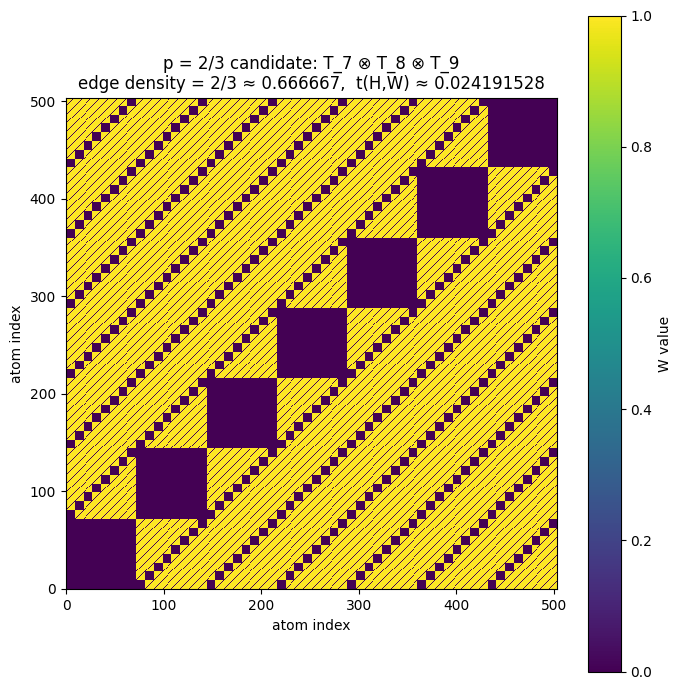
\includegraphics[width=\textwidth]{tensor_turan_T7_T8_T9.png}
    \caption{$T_7\otimes T_8\otimes T_9$, $e(W)=2/3$.}
\end{subfigure}
\hfill
\begin{subfigure}{0.32\textwidth}
    \centering
    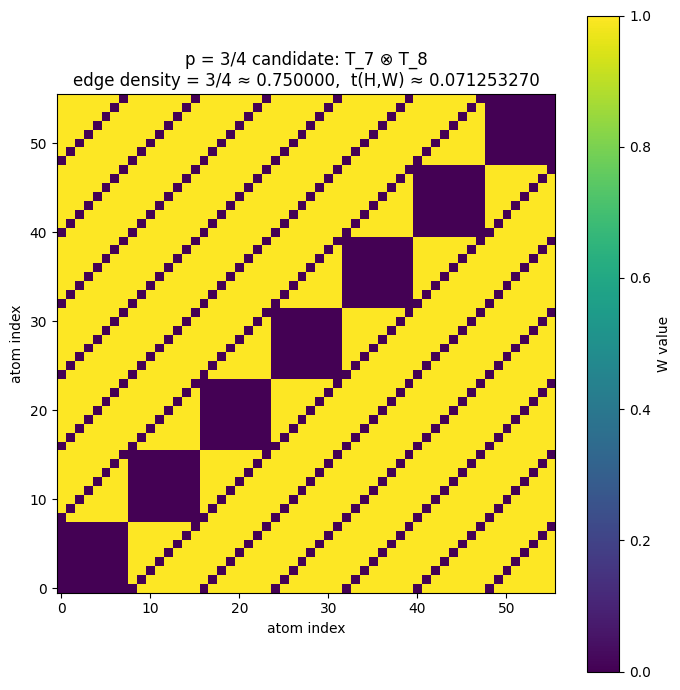
\includegraphics[width=\textwidth]{tensor_turan_T7_T8.png}
    \caption{$T_7\otimes T_8$, $e(W)=3/4$.}
\end{subfigure}
\hfill
\begin{subfigure}{0.32\textwidth}
    \centering
    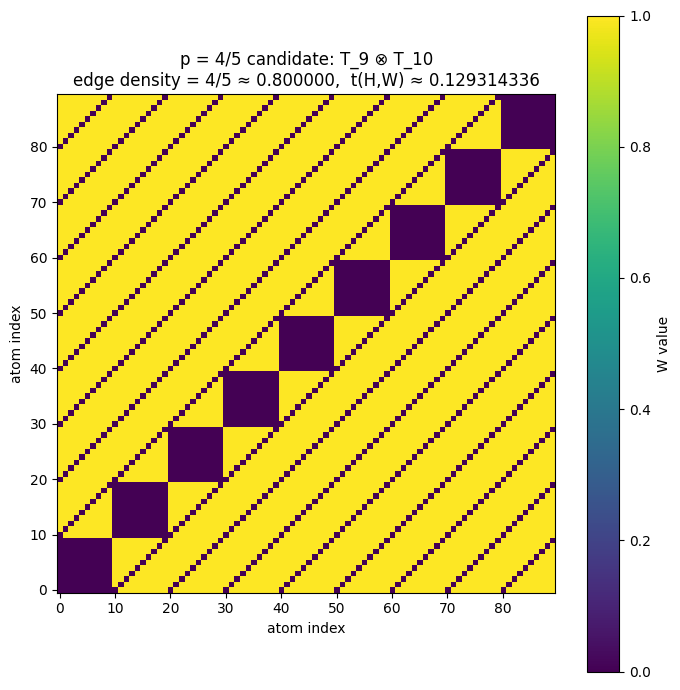
\includegraphics[width=\textwidth]{tensor_turan_T9_T10.png}
    \caption{$T_9\otimes T_{10}$, $e(W)=4/5$.}
\end{subfigure}

\caption{Step-matrix visualisations of the tensor-product Tur\'an graphons.}
\end{figure}

\section{Conjectural interpretation}

The evidence suggests that the graph $H$ is minimised, at least for the first few Tur\'an densities, not by the constant graphon and not by the balanced complete $k$-partite graphon, but by higher-rank product structure. The tensor-product construction creates adjacency only when all Tur\'an coordinates differ. This generates a large, organised set of non-edges while preserving the target edge density.

A natural conjectural picture is therefore
\[
\phi_H(2/3)
\stackrel{?}{=}
t(H,T_7\otimes T_8\otimes T_9),
\]
\[
\phi_H(3/4)
\stackrel{?}{=}
t(H,T_7\otimes T_8),
\]
and
\[
\phi_H(4/5)
\stackrel{?}{=}
t(H,T_9\otimes T_{10}).
\]
A rigorous proof would likely require a flag-algebra certificate or an equivalent graphon variational argument.

\end{document}